% The block of the encoder and of the forecaster (Section "Encoder and
% forecaster"). Build: pdflatex arch_block.tex  ->  arch_block.pdf
% Checked against src/blocks.py at 6674dc92 (the run "grey"): the conv
% feeds only the attention branch, whose residual adds to the stream as it
% was before the conv; pre-norm FFN; no final norm before the sphere.
% Colours: the convention of the Transformer figure (attention orange,
% feed-forward blue, normalisation yellow), as Okabe-Ito tints at 55%.
% Under simulated protanopia, deuteranopia and tritanopia, every pair of
% fills keeps a CIELAB distance of at least 11, and black text keeps a
% contrast of at least 10.8:1. The labels name every type, so no reading
% depends on colour alone.
\documentclass[tikz,border=1pt]{standalone}
\usepackage[T1]{fontenc}
\usepackage{amsmath}
\usetikzlibrary{positioning,arrows.meta,fit,calc}
\definecolor{cconv}{HTML}{73CAB2}  % convolution: bluish green
\definecolor{cnorm}{HTML}{F7F097}  % normalisation: yellow
\definecolor{cattn}{HTML}{F1CA73}  % attention: orange
\definecolor{cffn}{HTML}{A2D6F3}   % feed-forward: sky blue
\begin{document}
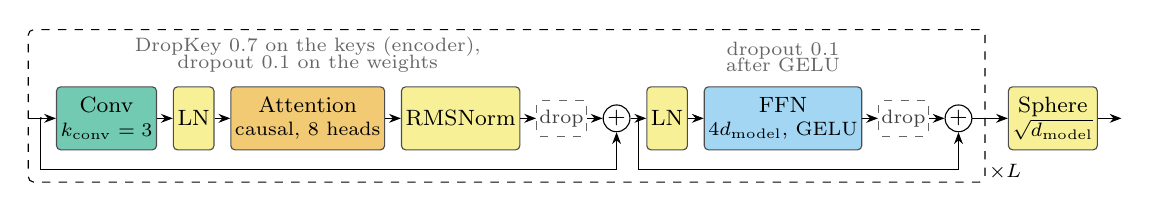
\begin{tikzpicture}[
  font=\footnotesize,
  node distance=2mm,
  box/.style={draw=black!70, rounded corners=1.5pt, align=center, inner sep=1.5pt,
    minimum height=8mm},
  op/.style={draw, circle, inner sep=0pt, minimum size=3.4mm},
  arr/.style={-{Stealth[length=1.5mm]}},
  drop/.style={draw=black!60, dashed, rounded corners=1pt, inner sep=1pt,
    font=\scriptsize, text=black!75, minimum height=4.5mm},
  note/.style={font=\scriptsize, text=black!60, align=center},
]
  \coordinate (in);
  \node[box, fill=cconv, right=3.5mm of in] (conv) {Conv\\[-1pt]{\scriptsize $k_{\mathrm{conv}} = 3$}};
  \node[box, fill=cnorm, right=of conv] (ln1) {LN};
  \node[box, fill=cattn, right=of ln1] (att) {Attention\\[-1pt]{\scriptsize causal, $8$ heads}};
  \node[box, fill=cnorm, right=of att] (rms) {RMSNorm};
  \node[drop, right=of rms] (dp1) {drop};
  \node[op, right=of dp1] (add1) {$+$};
  \node[box, fill=cnorm, right=of add1] (ln2) {LN};
  \node[box, fill=cffn, right=of ln2] (ffn) {FFN\\[-1pt]{\scriptsize $4d_{\mathrm{model}}$, GELU}};
  \node[drop, right=of ffn] (dp2) {drop};
  \node[op, right=of dp2] (add2) {$+$};
  \node[box, fill=cnorm, right=4.5mm of add2] (sph) {Sphere\\[-1pt]{\scriptsize $\sqrt{d_{\mathrm{model}}}$}};
  \coordinate[right=3mm of sph] (out);

  \draw[arr] (in) -- (conv);
  \foreach \a/\b in {conv/ln1, ln1/att, att/rms, rms/dp1, dp1/add1, add1/ln2,
                     ln2/ffn, ffn/dp2, dp2/add2, add2/sph, sph/out}
    \draw[arr] (\a) -- (\b);

  % Residual paths, under the boxes.
  \coordinate (s1) at ($(in)!0.45!(conv.west)$);
  \draw[arr] (s1) -- ++(0, -6.5mm) -| (add1.south);
  \coordinate (s2) at ($(add1.east)!0.5!(ln2.west)$);
  \draw[arr] (s2) -- ++(0, -6.5mm) -| (add2.south);
  \fill (s1) circle (0.5pt);
  \fill (s2) circle (0.5pt);

  % Regularisation during training.
  \node[note, above=0.6mm of att] {DropKey $0.7$ on the keys (encoder),\\[-2pt] dropout $0.1$ on the weights};
  \node[note, above=0.6mm of ffn] {dropout $0.1$\\[-2pt] after GELU};

  % The block repeats L times.
  \coordinate (lo) at ($(s1) + (0, -6.5mm)$);
  \coordinate (hi) at ($(att.north) + (0, 5.6mm)$);
  \node[draw, dashed, rounded corners=2pt, inner sep=1.6mm,
        fit=(conv) (add2) (lo) (hi)] (blk) {};
  \node[note, anchor=south west, text=black, inner sep=1pt] at (blk.south east)
        {$\times L$};
\end{tikzpicture}
\end{document}
